\chapter{Experimental Setup}
\label{ch:setup}



\noindent In this chapter, the system setup is defined.
%The platform adopted is shown, then a brief description is provided of both the hardware and the software exploited to provide the specified features.
An overview of the platform adopted with its rationale is followed by the description of both hardware and software solutions exploited.

\section{Overview}
\label{sec:over-system}

\noindent
The system will be built upon the \Gls{HRP}~\cite{HRP}, a \Gls{ROS} enabled Husqvarna Automower 450X providing access to information of control commands, wheel encoder measurements, and GPS position estimates.
It has been improved by a former thesis student~\cite{HRPTianze} and it is now equipped with additional two \Glspl{IMU} and a \Gls{RGBD} camera, as shown in Figure \ref{fig:HardwareSetup}.
\begin{figure}[!ht]
	\begin{center}
		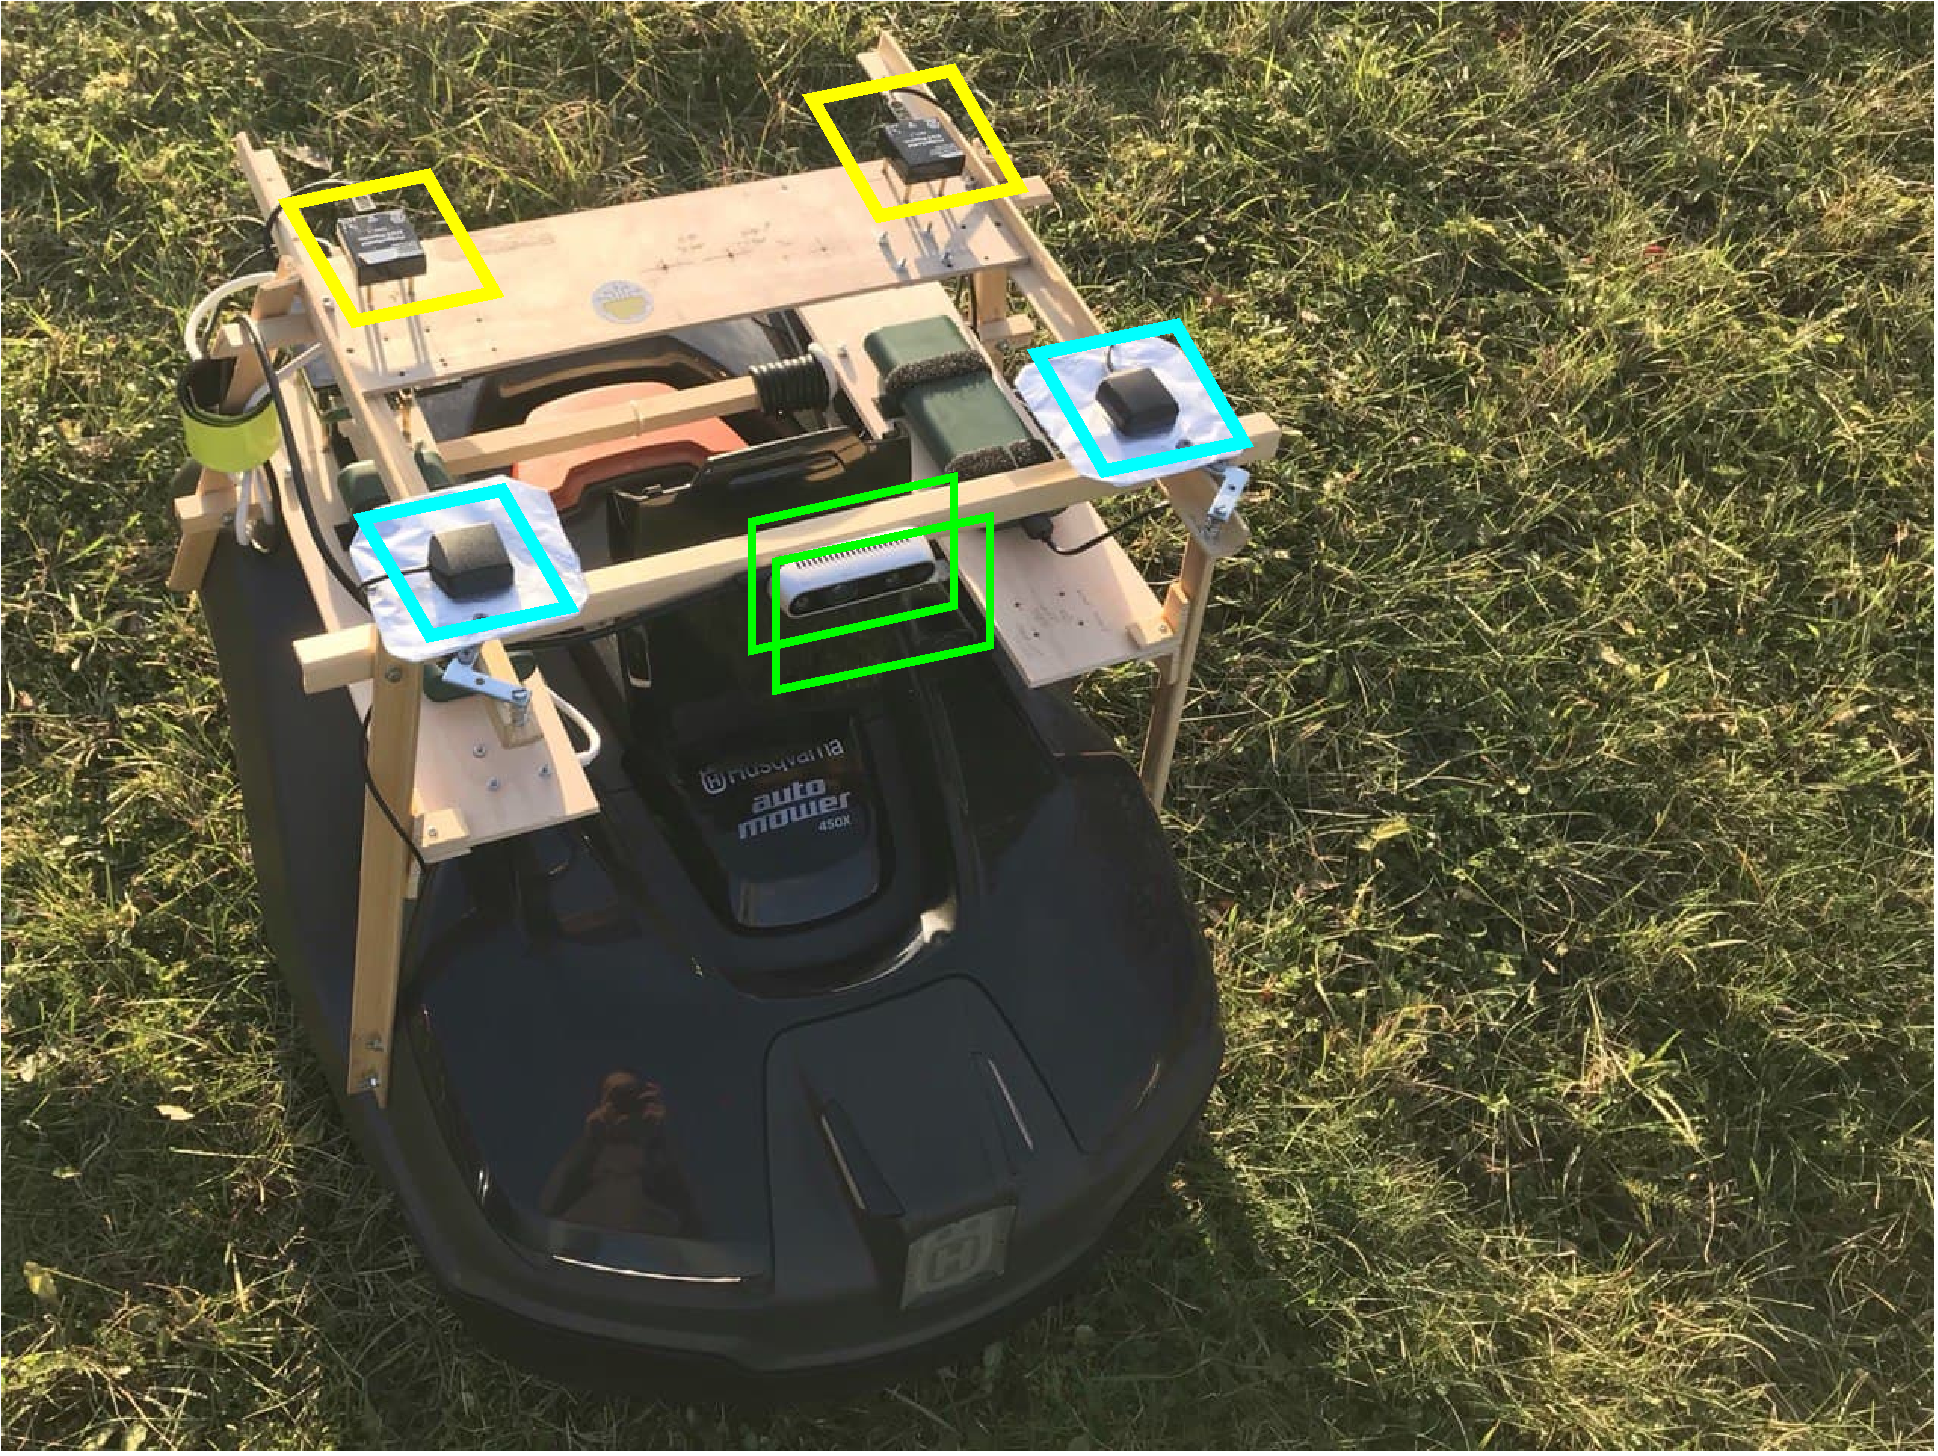
\includegraphics[clip, trim=0.5cm 0.6cm 8.5cm 0.6cm , width=0.45 \textwidth]{Images/1-Introduction/projectTheme.pdf}
		\caption{
			\gls{ALM} Model with focus on additional sensors:\\
			\glspl{IMU} [yellow], extra \gls{GNSS} receivers (not relevant) [cyan], and Camera [green].
			\centering }
		\label{fig:HardwareSetup}
	\end{center}
\end{figure}


\com{
\subsection{Scope}
Describe the boundary/limits of your thesis project and what you are explicitly not going to do. This will help you bound your efforts – as you have clearly defined what is out of the scope of this thesis project. Explain the delimitations. These are all the things that could affect the study if they were examined and included in the degree project.
\noindent
}

Since \glspl{ALM} are consumer products, some constraints will be taken into account. %, such as the configuration complexity and the sensors' cost analysis.
Those elements provide the rationale for this project to focus on some aspects rather than others.
Some of them are directly limiting and they are not going to be investigated further.
Some others instead will be included in the future works, discussed at the end of this thesis.
The most relevant are described below:
\begin{itemize}
    \item The operation area is projected into a \Gls{2D} environment. This allows for an initial definition for the localisation and mapping, and it could be expanded to \gls{3D} only after this phase has been refined.  
    \item The usage of an embedded device, such as a \gls{RPi}, limits the computational power of the module. Thus, the performance might not be as good as if a more powerful device would be used. %In this project, this aspect of optimization of the limited resources available on an embedded system will not be investigate.
    %\\~\\
    \item A complete \gls{SLAM} algorithm is too computationally expensive to perform well in real-time, considering the dynamic outdoor environment and the limited computational power.
    The proposed approach is to split the two different phases.
    The localisation aspect will be achieved with a sensor fusion approach. The mapping simply uses its resulting pose to update its map using eventual collision events.%receiving directly a predefined map layout configuration of the environment with a given starting point of the \gls{ALM} should ease the process of  within it.
    \item Relying on a camera in outdoor settings means that the weather conditions and time of mowing can affect the results.
    As such, the testing will be performed in similar configurations, and, if possible, with an attitude towards limiting this issue.
    \item A Range Finder Sensor, e.g., lidar, was not considered as most of the outdoor environment will be either sparse or empty.
    Thus, the sensor would not be able to provide valuable improvement to justify the expensive choice.
    Moreover, such a sensor requires a relevant amount of computational power to be run.
\end{itemize}


%The two additional \gls{GNSS} receivers have not been exploited as they provide poor performances.

\section{Hardware}
\label{sec:system}

\noindent
The proposed architecture is based on the \gls{HRP}, with its original board and sensors, with the addition of a Raspberry Pi 4, which provides higher computational performance, and additional sensors to capture additional phenomena used by the localisation module.
The proposed architecture is defined in Figure \ref{fig:hard-conf}.
%The original board is tasked to guide the \gls{ALM} and make him move according to the desired path, also at the end the \gls{ALM} was free to run its random path and use the algorithm implemented to stay inside the boundaries.


\begin{figure}[!ht]
	\begin{center}
		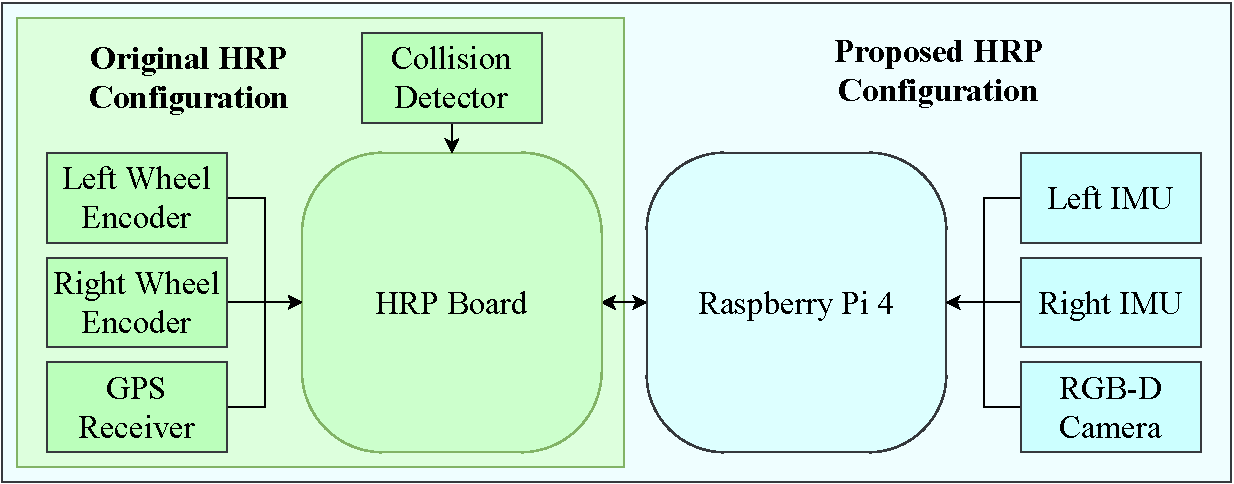
\includegraphics[width=1 \textwidth]{Images/3-0-SetUp/HWSetUp.pdf}
		\caption{Hardware Configuration including computational systems(rounded) and sensors(squared) of the original platform(green) with the updated version(blue). \centering }
		\label{fig:hard-conf}
	\end{center}
\end{figure}


%\subsection{HRP Board}
%\noindent 
The main board of the \gls{HRP} is a STM32-based microcontroller, shown in Figure \ref{fig:hrp-board}.
It is used to provide basic features for the \gls{ALM}, e.g., wheel control and collision detection. 
For the specific case of the \gls{HRP}, Husqvarna has provided an USB interface to connect it to external host computers, allowing for the connection with the Raspberry Pi 4 module.
\begin{figure}[!ht]
	\begin{center}
			\begin{center}
				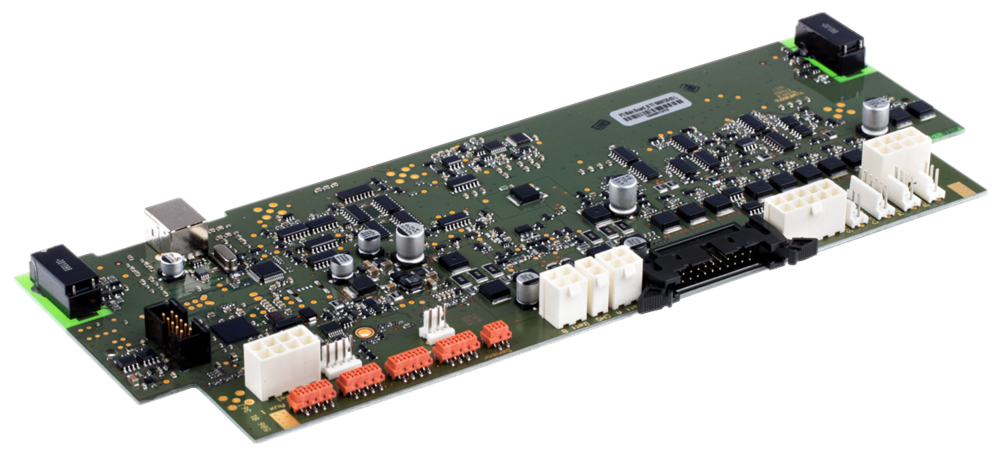
\includegraphics[width=0.5\textwidth]{Images/3-0-SetUp/586813503.png}
			\end{center}
			\caption{\gls{HRP} Main board.}
			\label{fig:hrp-board}
	\end{center}
\end{figure}

%\subsection{Raspberry Pi 4}
%\noindent 
The Raspberry Pi 4 Model B has been chosen as host computer, as shown in Figure \ref{fig:rpi4}.
It has been added to supplement the \gls{HRP} board, providing additional computational power for the implementation of additional features, i.e., the localisation and mapping modules. 
Moreover, additional hardware such as the \glspl{IMU}, and the \gls{RGBD} camera have been directly connected to it to improve the final \gls{HRP} configuration.
This platform is the one which will be used to guide the \gls{ALM}.
\begin{figure}[!ht]
	\begin{center}
			\begin{center}
				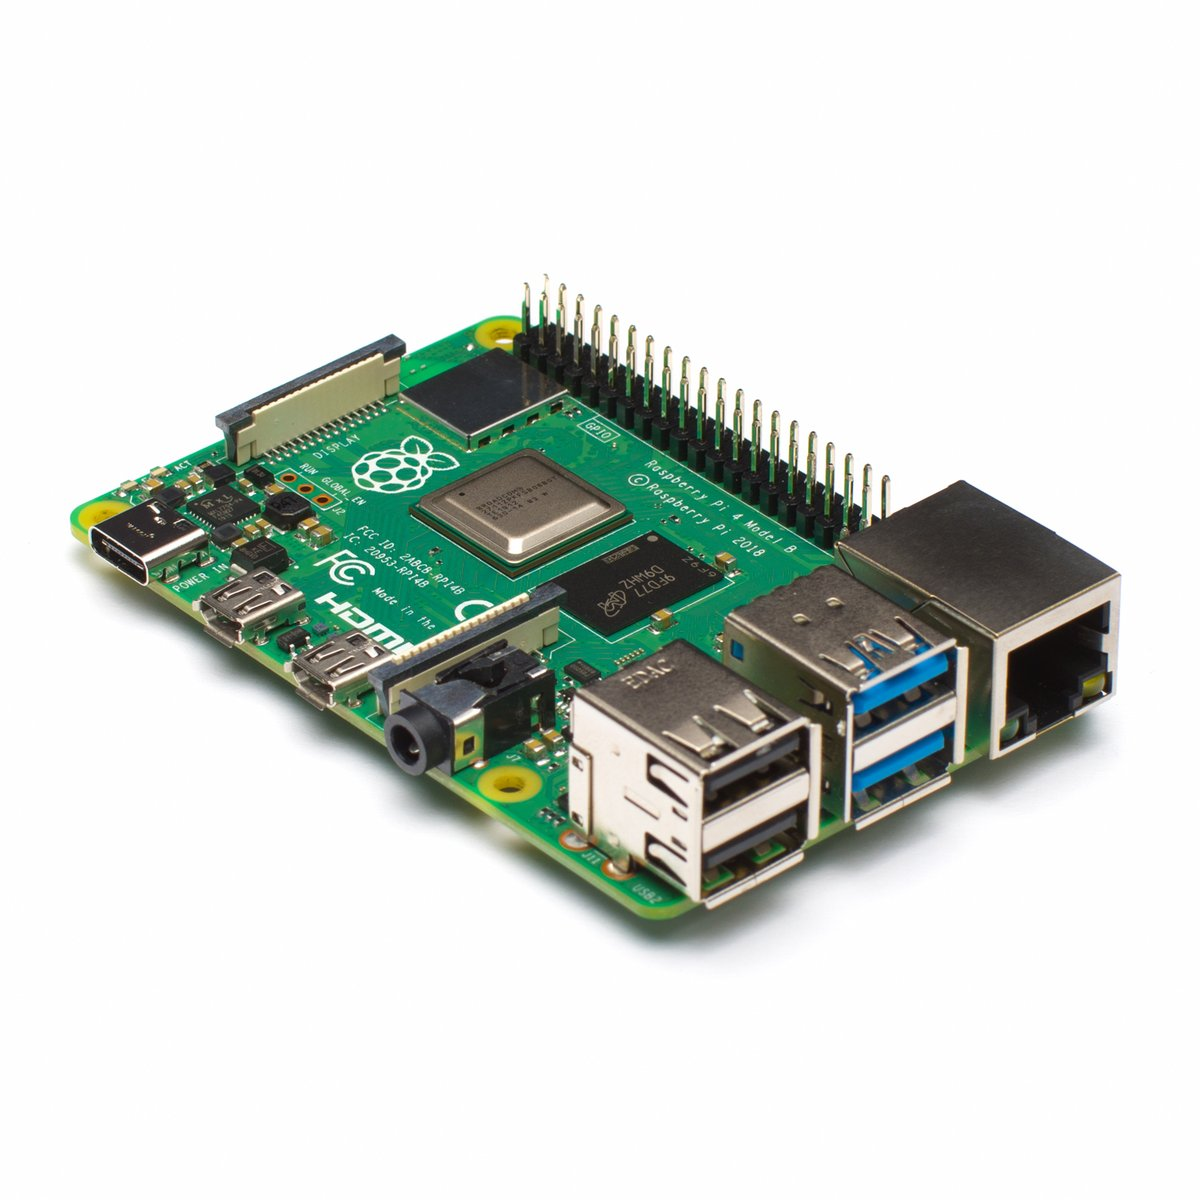
\includegraphics[clip, trim=2cm 8cm 2cm 10cm , width=0.5\textwidth]{Images/4-Methods/RPi4.jpg}
			\end{center}
			\caption{Raspberri Pi 4 Model B.}
			\label{fig:rpi4}
	\end{center}
\end{figure}

%\subsection{Wheel Encoders}
%\noindent
The wheel encoders are included in both of the motors of the wheels of the \gls{ALM}, inside the Motor Kit shown in Figure \ref{fig:wheel}.
They measure the wheel displacement and they provide \gls{WO} through estimates of the wheel velocities used to derive the related linear and angular velocities of the \gls{ALM}.
They work at a frequency of \SI{200}{Hz}.
\begin{figure}[!ht]
	\begin{center}
			\centering
			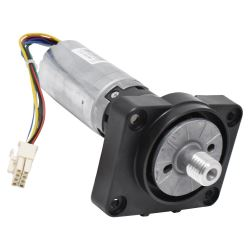
\includegraphics[width=0.30\textwidth]{Images/4-Methods/MotorEnc.jpeg}
			\caption{Motor Kit for Automower 450X.}
		\label{fig:wheel}
	\end{center}
\end{figure}


%\subsection{GPS Receiver}
%\noindent
A \gls{GPS} receiver is directly embedded in the automower as part of the Connect Kit developed by Husqvarna for positioning purposes, as shown in Figure \ref{fig:gps-module}.
It is available for the advanced \gls{ALM} model the \gls{HRP} is built upon and it is mounted on the center of the \gls{HRP}, as per assembly instructions.
Its full specifications have not been disclosed by the \gls{ALM} producer, but it can be said that it is a combined sensor with loosely coupled GNSS-INS integration, i.e., it uses both measurements from an internal \gls{IMU} sensor and the \gls{GPS} receiver to provide more reactive position fixes. 
Its measurements are derived using the computations of pseudoranges obtained from the \gls{GPS} receiver and fusing them with the measurements of an \gls{INS}, as such, consecutive measurements are correlated.
%TODO
% Better define the Loosely Coupled GNSS-INS Integration not disclosed by the \gls{ALM} producer
It works at a frequency of \SI{1}{Hz} and it is the only sensor which directly provides the measurements related to the pose states of position and orientation.
\begin{figure}[!ht]
	\begin{center}
			\begin{center}
				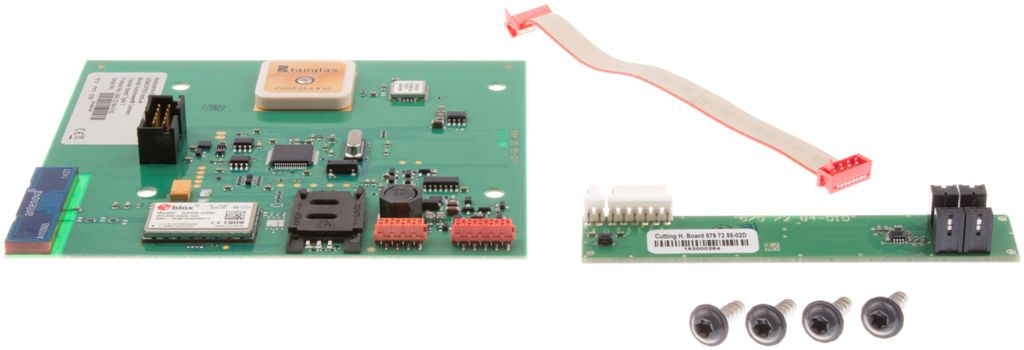
\includegraphics[width=0.75\textwidth]{Images/3-0-SetUp/Husqvarna_Automower_Connect_module_2.jpeg}
			\end{center}
			\caption{Husqvarna Automower Connect module.}
			\label{fig:gps-module}
	\end{center}
\end{figure}


%\subsection{IMUs}
%\noindent
The additional \glspl{IMU} adopted are the PhidgetSpatial Precision 3/3/3 High Resolution, shown in Figure \ref{fig:spatial}.
They are mounted on the structure of the \gls{HRP} in position [$x=0$\SI{}{cm}, $y=\pm16$\SI{}{cm}, $z= 37$\SI{}{cm}] and orientation [$\theta_z=0$\SI{}{rad}] with respect to the robot coordinate frame $P_R$.
They include gyroscopes, accelerometers, and compasses on each of the 3-axis.
The measurements of angular velocity and linear acceleration are used, respectively, to improve the orientation estimates and to model the noise of the prediction step.
It provides angular velocity and linear acceleration at a frequency of \SI{250}{Hz}.
\begin{figure}[!ht]
	\begin{center}
			\begin{center}
				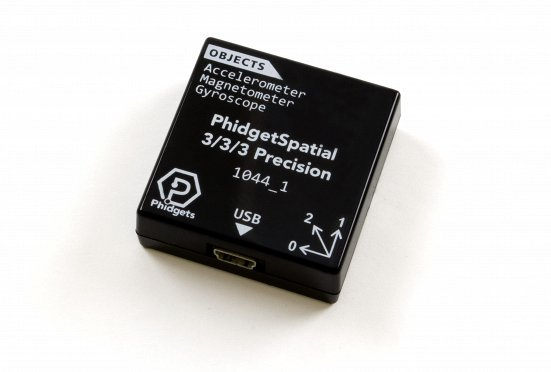
\includegraphics[width=0.5\textwidth]{Images/4-Methods/1044_1B.jpg}
			\end{center}
			\caption{IMU Sensor.}
			\label{fig:spatial}
	\end{center}
\end{figure}



%\subsection{RGB-D Camera}
%\noindent 
The device adopted is the Intel® RealSense™ depth camera D435, shown in Figure \ref{fig:camera_sensor}.
It is mounted on the structure of the \gls{HRP} in position [$x=0.23$\SI{}{cm}, $y=0$\SI{}{cm}, $z= 33$\SI{}{cm}] and orientation [$\theta_z=0$\SI{}{rad}] with respect to the robot coordinate frame $P_R$.
It provides \gls{RGBD} images through a stereo camera, i.e., both \gls{RGB} and Depth information.
The images it provides are used to generate the \gls{VO} estimates, bases on the displacements of features identified in consecutive shots.
It is used to provide velocity measurements through \gls{VO} at a frequency of \SI{5}{Hz}.
\begin{figure}[!ht]
	\begin{center}
			\begin{center}
				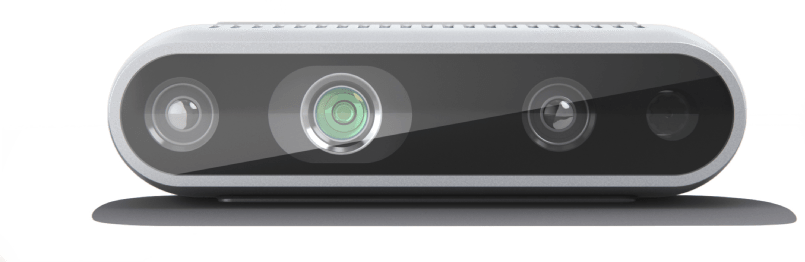
\includegraphics[width=0.5\textwidth]{Images/4-Methods/d435i-1.png}
			\end{center}
		\caption{Camera.}
		\label{fig:camera_sensor}
	\end{center}
\end{figure}


%\subsection{Collision Sensors}
%\noindent
The collision sensors, one of which is shown in Figure \ref{fig:collision_sensor}, detect when the frame of the automower has been in contact with an object.
They fire an event whenever the external frame bumps with an object and consequently reach the touch sensors positioned on the back of the wheels.
Thus, they allow for the detection of the objects and they are used to update the knowledge of the map.
\begin{figure}[!ht]
	\begin{center}
			\begin{center}
				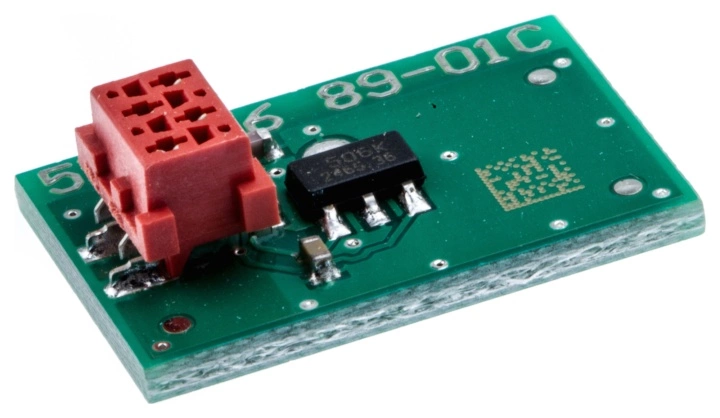
\includegraphics[width=0.5\textwidth]{Images/3-0-SetUp/Collision.png}
			\end{center}
		\caption{Circuit board collision sensor.}
		\label{fig:collision_sensor}
	\end{center}
\end{figure}


\section{Software}
\label{sec:soft-system}
\noindent The following software modules are adopted to code the required features.

As the \gls{HRP} is a \gls{ROS}-enabled platform, its latest available version has been used, namely, ROS Noetic.
For its installation, the Ubuntu operating system 20.04 has been choosen for the Raspberry Pi 4, instead the \gls{HRP} board runs a proprietary software which is not disclosed, but its program modules are written in C++ and they interface with ROS.
The software languages which have been used are C++11 for both the internal software and the hardware related tasks, such as the controller of the \gls{HRP} and the sensor's drivers.
Python 3.8 has been chosen for the high level tasks identified, such as the localisation and mapping modules developed as main contributions.
The different software modules are structured using \gls{ROS} nodes, which are sharing data using specific \gls{ROS} topics. An overview of the \gls{ROS} framework is available in Appendix \ref{ch:ros}. 

\cleardoublepage